\documentclass{beamer}
% Required packages
\usepackage{amsmath}
\usepackage{physics}
\usepackage{graphicx}
\usepackage{siunitx}
\usepackage{xcolor}
\graphicspath{{../images/}}
% Define custom colors for DS9 theme
\definecolor{ds9blue}{RGB}{25,25,112}
\definecolor{ds9gold}{RGB}{218,165,32}
\definecolor{ds9grey}{RGB}{105,105,105}
\definecolor{ds9red}{RGB}{178,34,34}
% Set up the Madrid theme with custom colors
\usetheme{Madrid}
\usecolortheme{whale}
\setbeamercolor{palette primary}{bg=ds9blue,fg=white}
\setbeamercolor{palette secondary}{bg=ds9grey,fg=white}
\setbeamercolor{palette tertiary}{bg=ds9gold,fg=black}
\setbeamercolor{palette quaternary}{bg=ds9red,fg=white}
\setbeamercolor{structure}{fg=ds9blue}
\setbeamercolor{title}{fg=ds9gold}
\setbeamercolor{subtitle}{fg=ds9gold}
\setbeamercolor{frametitle}{bg=ds9blue,fg=white}
\setbeamercolor{block title}{bg=ds9blue,fg=white}
\setbeamercolor{block body}{bg=ds9grey!20,fg=black}

\title[CH 1.3]{PHYS11 CH:1.3}
\subtitle{The Language of Physics: Physical Quantities and Units}
\author[Mr. Gullo]{Mr. Gullo}
\date[Sept 2025]{September 5, 2025}

\begin{document}

\begin{frame}
    \titlepage
    \centering
\end{frame}

\begin{frame}
    \frametitle{Outline}
    \tableofcontents
\end{frame}

\section{Learning Objectives}
\begin{frame}
    \frametitle{Learning Objectives}
    By the end of this section, you will be able to:
    \pause
    \begin{itemize}
        \item Associate physical quantities with their International System of Units (SI) and perform conversions among SI units using scientific notation.
        \pause
        \item Relate measurement uncertainty to significant figures and apply the rules for using significant figures in calculations.
        \pause
        \item Correctly create, label, and identify relationships in graphs using mathematical relationships (e.g., slope, y-intercept).
    \end{itemize}
\end{frame}

\section{Key Concepts}
\begin{frame}
    \frametitle{SI Units \& Scientific Notation}
    \begin{block}{Physical Quantities and Units}
        Physics relies on making measurements, which are expressed in terms of \textbf{units}.
        \pause
        \begin{itemize}
            \item \textbf{Base Units:} The seven fundamental units of the SI system (meter, kilogram, second, ampere, kelvin, mole, candela).
            \pause
            \item \textbf{Derived Units:} Combinations of base units (e.g., speed in \(\text{m/s}\)).
        \end{itemize}
    \end{block}
    \pause
    \begin{block}{Scientific Notation}
        A method for writing very large or small numbers.
        \pause
        \begin{itemize}
            \item Format: \(x \times 10^y\)
            \pause
            \item Example: The number \(840,000,000,000,000\) is written as \(8.40 \times 10^{14}\).
            \pause
            \item The power of 10 is called the \textbf{order of magnitude}.
        \end{itemize}
    \end{block}
\end{frame}

\begin{frame}
    \frametitle{Accuracy, Precision, and Uncertainty}
    \begin{columns}
        \begin{column}{0.5\textwidth}
            \begin{block}{Definitions}
                \begin{itemize}
                    \item \textbf{Accuracy:} How close a measurement is to the correct or accepted value.
                    \pause
                    \item \textbf{Precision:} How well repeated measurements generate the same or similar results.
                    \pause
                    \item \textbf{Uncertainty:} A "disclaimer" for your measured value, often written as a \(\pm\) amount. E.g., \(11.0 \pm 0.2\) inches.
                \end{itemize}
            \end{block}
        \end{column}
        \begin{column}{0.5\textwidth}
            \begin{figure}
    \centering
    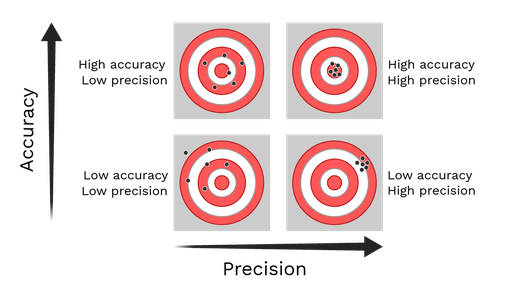
\includegraphics[width=0.8\linewidth]{phys11-accuracy-precision-targets.png}
    \caption{Four targets showing different combinations of accuracy and precision}
\end{figure}
        \end{column}
    \end{columns}
\end{frame}

\begin{frame}
    \frametitle{Significant Figures}
    \begin{block}{What are they?}
        The number of significant figures in a measurement indicates the \textbf{precision} of the measuring tool. It includes all digits measured reliably plus one estimated digit.
    \end{block}
    \pause

    \begin{figure}
        \centering
        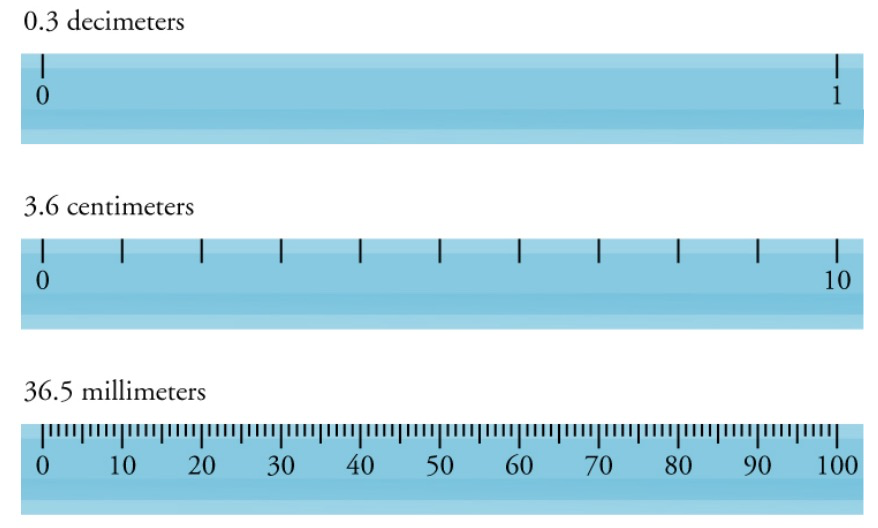
\includegraphics[width=0.8\linewidth]{phys11-rulers-significant-figures.png}
        \caption{Three rulers showing different levels of measurement precision}
    \end{figure}
\end{frame}

\begin{frame}
     \begin{figure}
        \centering
        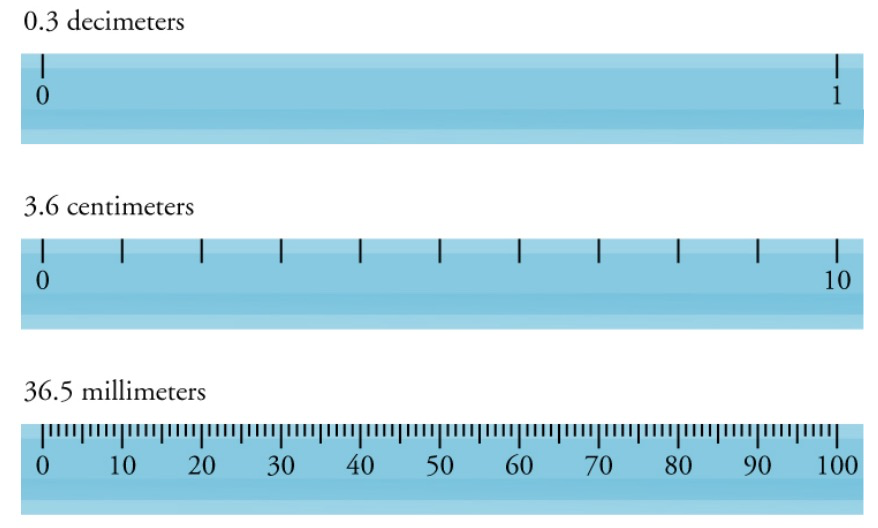
\includegraphics[width=0.8\linewidth]{phys11-rulers-significant-figures.png}
    \end{figure}
    \begin{block}{Rules for Zeros}
        \begin{itemize}
            \item Zeros between non-zero digits are significant (e.g., 101 has 3 sig figs).
            \pause
            \item Leading zeros are not significant (e.g., 0.053 has 2 sig figs).
            \pause
            \item Trailing zeros are ambiguous. Use scientific notation to clarify (e.g., \(1.30 \times 10^3\) has 3 sig figs, while \(1.3 \times 10^3\) has 2).
        \end{itemize}
    \end{block}
\end{frame}

\section{Equations and Rules}
\begin{frame}
    \frametitle{Key Equations \& Calculation Rules}
    \begin{block}{Percent Uncertainty}
        One method of expressing uncertainty is as a percent of the measured value.
        \pause
        \[ \% \text{ uncertainty} = \frac{\delta A}{A} \times 100\% \]
        \pause
        Where \(A\) is the measurement and \(\delta A\) is the uncertainty in the measurement.
    \end{block}
    \pause
    \begin{block}{Rules for Significant Figures in Calculations}
        \begin{itemize}
            \item \textbf{Multiplication and Division:} The answer should have the same number of significant figures as the starting value with the \textit{fewest} significant figures.
            \pause
            \item \textbf{Addition and Subtraction:} The answer should have the same number of decimal places as the starting value with the \textit{fewest} decimal places.
        \end{itemize}
    \end{block}
\end{frame}

\section{Examples}
\begin{frame}
    \frametitle{I Do: Unit Conversion}
    \begin{exampleblock}{Problem: A Short Drive Home}
        Suppose you drive the \SI{10.0}{km} from your university to home in \SI{20.0}{min}. Calculate your average speed in (a) kilometers per hour (km/h) and (b) meters per second (m/s).
    \end{exampleblock}
    \pause
    \begin{block}{Solution (a): km/h}
        Average speed = \(\frac{\SI{10.0}{km}}{\SI{20.0}{min}}\). We need to convert minutes to hours.
        \pause
        \[ \text{speed} = \frac{\SI{10.0}{km}}{\SI{20.0}{min}} \times \left( \frac{\SI{60}{min}}{\SI{1}{h}} \right) = \SI{30.0}{km/h} \]
    \end{block}
    \pause
    \begin{block}{Solution (b): m/s}
        We can convert the result from part (a).
        \pause
        \[ \text{speed} = \frac{\SI{30.0}{km}}{\SI{1}{h}} \times \left( \frac{\SI{1000}{m}}{\SI{1}{km}} \right) \times \left( \frac{\SI{1}{h}}{\SI{3600}{s}} \right) = \SI{8.33}{m/s} \]
        \pause
        Note that all answers are given to three significant figures.
    \end{block}
\end{frame}

\begin{frame}
    \frametitle{We Do: Calculating Uncertainty}
    \begin{alertblock}{Problem}
        A bathroom scale reads a person's mass as \SI{65}{kg} with a \SI{3}{\percent} uncertainty. What is the uncertainty in their mass in kilograms? (Question 48)
    \end{alertblock}
    \pause
    \begin{block}{Setup}
        \begin{enumerate}
            \item Identify the given values:
            \begin{itemize}
                \item Mass \( (A) = \SI{65}{kg} \)
                \item Percent Uncertainty = \SI{3}{\percent}
            \end{itemize}
            \pause
            \item Start with the formula: \( \% \text{ uncertainty} = \frac{\delta A}{A} \times 100\% \)
            \pause
            \item Rearrange to solve for the uncertainty, \(\delta A\):
            \[ \delta A = \frac{\% \text{ uncertainty}}{100\%} \times A \]
        \end{enumerate}
    \end{block}
    \pause
    \begin{exampleblock}{Let's Solve It!}
        Now, plug in the numbers. What do you get for the uncertainty \(\delta A\)?
        \[ \delta A = \frac{3\%}{100\%} \times \SI{65}{kg} = \textbf{?} \]
        \pause
        The answer is \SI{1.95}{kg}, which we can round to \SI{2}{kg} (Option a).
    \end{exampleblock}
\end{frame}

\begin{frame}
    \frametitle{You Do: Metric Prefixes}
    \begin{alertblock}{Problem}
        Which of the following would describe a length that is \(2.0 \times 10^{-3}\) of a meter? (Question 47)
    \end{alertblock}
    \pause
    \begin{itemize}
        \item[a.] \SI{2.0}{kilometers}
        \pause
        \item[b.] \SI{2.0}{megameters}
        \pause
        \item[c.] \SI{2.0}{millimeters}
        \pause
        \item[d.] \SI{2.0}{micrometers}
    \end{itemize}
    \pause
    \begin{block}{Hint}
        What metric prefix corresponds to the factor \(10^{-3}\)?
    \end{block}
    \pause
    \begin{beamercolorbox}[rounded=true,center,wd=\textwidth]{block body}
        The correct answer is \textbf{c. \SI{2.0}{millimeters}}. The prefix "milli-" means \(10^{-3}\).
    \end{beamercolorbox}
\end{frame}

\section{Summary}
\begin{frame}
    \frametitle{Summary}
    \begin{itemize}
        \item Physics is a quantitative science, requiring a standard system of units (SI units).
        \pause
        \medskip
        \item \textbf{Accuracy} is about correctness, while \textbf{precision} is about consistency.
        \pause
        \medskip
        \item \textbf{Significant figures} communicate the precision of our measurements and must be handled correctly in calculations.
        \pause
        \begin{itemize}
            \item Multiplication/Division: Fewest total sig figs.
            \pause
            \item Addition/Subtraction: Fewest decimal places.
        \end{itemize}
        \pause
        \medskip
        \item \textbf{Unit conversion} is a fundamental skill used to ensure calculations are performed with consistent units.
    \end{itemize}
\end{frame}

\end{document}